% ====================================================================
% PRL-style paper draft. Build: latexmk -pdf main_paper.tex
% The companion analysis note contains the complete validation record,
% technical details, extended-fiducial study, and PET methodology.
% ====================================================================
\documentclass[aps,prl,reprint,superscriptaddress,nofootinbib]{revtex4-2}

\usepackage[T1]{fontenc}
\usepackage{amsmath,amssymb}
\usepackage{graphicx}
\usepackage{microtype}
\usepackage{siunitx}
\usepackage{xcolor}
\usepackage[colorlinks=true,allcolors=blue!55!black]{hyperref}

\graphicspath{{figures/}}
\DeclareGraphicsExtensions{.pdf}
\newcommand{\pT}{p_{T}}
\newcommand{\pPar}{p_{\parallel}}
\newcommand{\Eavail}{E_{\mathrm{avail}}}

% ====================================================================
% values.tex --- SINGLE SOURCE OF TRUTH for every headline number that
% recurs across the build (abstract / executive summary / body section).
% Edit a result HERE and it updates in all three PDFs.
% Numbers that appear exactly once (deep in a section, a table,
% or App. B) are NOT macroized here -- they cannot drift, so they stay inline
% at their single site.
%
% Convention: cross sections carry their full value+exponent so \SI expands
% cleanly (e.g. \SI{\sigTwoD}{cm^2/nucleon}); ratios/percentages/significances
% are bare numbers (e.g. \SI{\uqMedian}{\percent}, $\ratioTot$).
% ====================================================================

% --- 2D reproduction (the demonstrator) ---
% PROVENANCE, ADDED 2026-08-21 (OI-130). These three were the HARD CORE of the OI-130
% enumeration: of 71 macros they were the only ones naming NO backing artifact anywhere, even
% under the generous bound -- which makes them UNBINDABLE BY CONSTRUCTION, since no hash-binding,
% freeze gate or receipt check can fire on a macro that cites no path. They are the most-quoted
% numbers in the note, so that was the worst place for the gap to be.
%   PRODUCER  2d-unfolding/agreement_windows_receipt.py
%   RECEIPT   docs/orchestration/receipts/RECEIPT-2d-agreement-windows-20260821.json
%   RUN       saul, ROOT 6.28/12, at git 5996eb29
%   ARTIFACTS ours  hXSec2D             from 2d-unfolding/2d_crossSection_omnifold_MEFHC_5iter.root
%                                       sha256 142a45b0efc753d91e95376c28ac3f6a477d582014a919e49d6d71079a127fd5
%             paper pt_pl_cross_section  from minerva_paper_anc/cov_ptpl_minerva_inclusive_6GeV.root
%                                       sha256 6c6dce72050bb8f128fab8e286349b250bc60d1c767e162bf15a0f009f3573e3
%   MEASURED  integral ours 3.0733e-38; paper 3.0390e-38; ratio 1.0113
% THE TOTAL IS AN INTEGRAL, NOT A SUM OF BIN CONTENTS, and getting that wrong is easy here: these
% histograms hold d2sigma/(dpT dp_par), so the bin-area Jacobian is required. Measured without it,
% the sums came out 12.14x these values -- THE SAME FACTOR ON BOTH FILES -- while the RATIO still
% reproduced, because the Jacobian cancels. A ratio agreeing is not evidence that its operands do;
% the receipt keeps both numbers so nobody repeats it.
% STILL NOT ESTABLISHED: that this producer is the method that ORIGINALLY produced these three, and
% both artifacts live on PURGEABLE SCRATCH and are untracked, so this closes the CITATION gap and
% not the DURABILITY one (OI-130's class, and OI-75 for the same shape elsewhere).
\newcommand{\sigTwoD}{3.073e-38}      % our 2D total; integral 3.0733e-38, receipt above
\newcommand{\sigTwoDpaper}{3.039e-38} % published 2D total; integral 3.0390e-38, receipt above
\newcommand{\ratioTot}{1.011}         % sigma_tot ours/paper; integral ratio 1.0113, receipt above
% PROVENANCE FOR THE NEXT FOUR MACROS -- RESOLVED 2026-08-21, AND THE HISTORY MATTERS.
% \medianBinRatio, \binsFive, \binsTen and \binsTwenty had NO committed producing script
% (OI-130). They were suppressed from all three deliverables on 2026-08-21 and are RESTORED
% here only because an authorized producer now attests them.
%   PRODUCER  2d-unfolding/agreement_windows_receipt.py
%   RECEIPT   docs/orchestration/receipts/RECEIPT-2d-agreement-windows-20260821.json
%   RUN       saul login34, ROOT 6.28/12, at git a3a4d3d1
%   MASK      205 of 224 bins, DERIVED as the positive diagonal of the paper ancillary's
%             StatOnlyCovariance on its own 224-bin global grid -- the same predicate
%             compare_to_paper_fullcov.py uses for its chi^2 ndf. The count is ASSERTED to be
%             205 and the producer exits 3 on any other value.
%   DENOM     205 of 205; ZERO bins excluded for a non-positive paper value, so the
%             denominator rule never bit and cannot be the source of the agreement.
%   INPUTS    ours  hXSec2D             from 2d_crossSection_omnifold_MEFHC_5iter.root
%                                       sha256 142a45b0efc753d91e95376c28ac3f6a477d582014a919e49d6d71079a127fd5
%             paper pt_pl_cross_section  from minerva_paper_anc/cov_ptpl_minerva_inclusive_6GeV.root
%                                       sha256 6c6dce72050bb8f128fab8e286349b250bc60d1c767e162bf15a0f009f3573e3
%   MEASURED  median 1.0064; 159/205 = 77.6 %; 193/205 = 94.1 %; 202/205 = 98.5 %
% ALL FOUR REPRODUCE THE PREVIOUSLY UNATTESTED VALUES EXACTLY. The producer was not aimed at
% them -- its receipt predeclares, in a field written before the run, that it attempts no
% reproduction and that a difference would be a finding.
% \medianBinRatio KEEPS ITS THREE-DECIMAL FORM: the receipt measures 1.0064 and 1.006 is that
% number at the precision the note has always printed. Changing the displayed precision would
% be a new editorial claim, not a restoration; the full value lives in the receipt.
% WHAT IS STILL NOT ESTABLISHED, and do not let the agreement blur it: this is not shown to be
% the method that ORIGINALLY produced these four. That provenance remains unrecoverable. OI-130's
% finding -- that no committed script reproduced the trio -- was TRUE OF THE TREE AS IT STOOD and
% stopped being true only when the producer landed.
% NOT THE PRODUCER, and the reason is worth keeping: 2d-unfolding/compare_to_paper_interior.py
% computes 5/10/20 % windows but masks to the STRICT INTERIOR (interior_mask(), pt_hi/pz_lo <=
% tan(20 deg)) intersected with the reported mask, so its denominators are SMALLER than 205
% (the audit's re-run reports 185/179/171/162/152/141). `git log --follow` puts that interior
% mask in the initial commit (d3239355), so no committed version of IT ever produced these.
% Any future change to these four goes through the producer and a fresh receipt.
\newcommand{\medianBinRatio}{1.006}   % median per-bin ratio ours/paper; receipt measures 1.0064, ATTESTED above
\newcommand{\binsFive}{77.6}          % percent of bins within 5%; 159/205, ATTESTED above
\newcommand{\binsTen}{94.1}           % within 10%; 193/205, ATTESTED above
\newcommand{\binsTwenty}{98.5}        % within 20%; 202/205, ATTESTED above
\newcommand{\pullMean}{0.089}
\newcommand{\pullRMS}{0.598}
\newcommand{\pullRMSr}{0.60}          % rounded, for prose
% FPS containment (Agent C WS1 statistical-validation repair, 2026-07-16):
% split-sample +/-1sigma truth-containment against an independent fixed NPZ truth.
% The estimator seed is fixed, so this diagnoses the statistical closure-toy
% stream, not the full adopted band. No aggregate binomial error is quoted.
\newcommand{\covFPS}{68.67}
\newcommand{\covNominal}{68.27}                              % Gaussian nominal
\newcommand{\covFPSanalytic}{77.6}   % FPS variant-A (independent C_stat): conservatively over-covers
\newcommand{\pullFrac}{68.71}        % OLD 2D "coverage" = same-ensemble pull fraction (diagnostic)
\newcommand{\pullMeanAbs}{0.794}\newcommand{\pullGauss}{0.798}  % <|r|> vs sqrt(2/pi)
\newcommand{\chiPaper}{3.66}          % chi2/ndf vs paper covariance
\newcommand{\chiCombined}{1.481}      % chi2/ndf vs combined (paper+ours) cov
\newcommand{\chiCombinedLog}{1.468}   % log-normal chi2/ndf, combined (paper+ours)
\newcommand{\chiCombinedSubStat}{11.56} % chi2/ndf, paper-stat-subtracted (over-corrects; secondary diagnostic)
% All three recomputed 2026-07-16 (compare_to_paper_fullcov.py, flux-fix hCov_combined
% [already incl. bootstrap] + ML). Supersede the pre-flux-fix appendix 1.699/1.688/23.96.

% --- uncertainty budget ---
\newcommand{\uqMedian}{6.87}          % our standalone combined median per-bin (%)
\newcommand{\uqPaper}{6.86}           % published total median per-bin (%)
\newcommand{\fluxBand}{4.99}          % leading flux band (%)
\newcommand{\rhoFluxMuon}{0.900}      % flux <-> muon-energy-scale correlation

% --- 3D / 4D higher-dimensional ---
\newcommand{\sigData}{3.07e-38}       % unfolded data total in the >=3D campaigns
\newcommand{\eavailMargin}{0.11}      % W-marginal recovers frozen 4D to this (%)
% Ascencio covariance metrics removed 2026-07-12: historical 4D covariance
% quarantined pending corrected production.

% (Eavail,W) significances removed 2026-07-12: historical covariance quarantined.
% Reintroduce macros only from a committed corrected-covariance ledger entry.

% --- corrected 5D GBDT candidate campaign; final active-lateral replacement pending ---
\newcommand{\gbdtFiveBlockMedian}{13.36}  % syst+stat+ML block sum, median/bin (%)
\newcommand{\gbdtFiveAdoptTrace}{5.81e-38} % adopted mean-centered sqrt(trace), xsec units
\newcommand{\gbdtFiveCVTrace}{6.24e-38}    % conservative CV-centered variant
\newcommand{\gbdtFiveMeanShift}{1.65e-38}  % separately reported joint mean-shift norm
\newcommand{\gbdtMlSplitTrace}{1.493e-39}  % adopted ML split-seed band sqrt(trace), xsec units
\newcommand{\gbdtAiEstTrace}{1.306e-39}    % fixed-data estimator-seed scan sqrt(trace), 12 seeds
\newcommand{\gbdtAiEstFrac}{87.5}          % estimator-only / split-varied sqrt-trace ratio (%)

% --- PET point-cloud track ---
% NOT QUOTABLE as current values -- niter=2 legacy. \petRatio is the quotient of two
% INLINE \SI{} literals in sec_pet.tex (2.796e-38 / 3.066e-38) that are not macros, so
% marking here cannot reach them; they are struck at the point of use instead. Both are
% struck wherever printed. Grounds: niter=2 vs the pinned niter=3 (CLM-010/CLM-012),
% the 2026-08-01 full-event estimator change, and J21 (no background subtraction).
% See docs/orchestration/INDEX-retracted-and-superseded-values.md.
\newcommand{\petRatio}{0.912}         % PET/GBDT absolute total ratio; niter=2 LEGACY, struck at use
\newcommand{\petClosure}{1}           % niter=2 LEGACY, struck at use; NOT QUOTABLE as a current value
% RULED 2026-08-21 BY JOSEPH -- the OPEN QUESTION recorded here on 2026-08-20 is CLOSED.
% Ruling: \petClosure is LEGACY and must not remain a current quantitative claim. The
% number and any present-tense "validates" language are removed from every print site.
% A qualitative statement may remain ONLY where it is explicitly labelled a legacy
% two-iteration self-consistency diagnostic. Basis:
% docs/orchestration/DETERMINATION-20260819-lanec-petclosure-is-legacy.md.
%
% Applied, and the treatment DIFFERS BY BUILD ON PURPOSE:
%   paper_body.tex (external paper, paper build only) -- REMOVED, and said so in the
%     prose. \dead{} is FORBIDDEN outside the note build and is checker-enforced, so an
%     outward-facing retraction is remove-and-say-so, never a strike.
%   sec_pet.tex:112 (note build only) -- STRUCK as $\sim$\,\dead{\SI{\petClosure}{\percent}}
%     with an explicit "struck: legacy two-iteration self-consistency diagnostic, not a
%     current validation" label, matching \dead{\petRatio} in that same caption.
%
% THE MACRO IS MARKED, NOT RETIRED, AND THAT IS DELIBERATE: sec_pet.tex still references
% it inside \dead{}, so deleting the definition would break the note build. Its comment
% now carries the same "niter=2 LEGACY, struck at use" marking as its two siblings --
% which is precisely the marking whose ABSENCE made its status undetermined before.
%
% The prior argument is preserved because it was sound and is now superseded rather than
% wrong: an ordinary-closure self-consistency check IS arguably a different object from an
% absolute PET-vs-GBDT comparison, so the niter=2 / full-event-estimator / J21 grounds do
% not obviously bite on it. That was an argument, not a ruling. The ruling supersedes it.
\newcommand{\petGbdtGap}{9}           % PET-vs-GBDT data-side gap (%); niter=2 LEGACY, struck at use
\newcommand{\petTotalMedian}{15.10}   % historical recoil-PET candidate; QUARANTINED
\newcommand{\petTotalTrace}{3.878e-38}% historical recoil-PET candidate; QUARANTINED
\newcommand{\petFourMedian}{12.37}    % historical recoil-PET 4D marginal; QUARANTINED
\newcommand{\petRetrainMedian}{4.18}  % targeted retraining-response median/bin (%)
\newcommand{\petLateralMedian}{2.11}  % PET-native frozen-map detector block (%)
% truth-cloud projection demonstration (reweight-then-project)
\newcommand{\pcHasCloud}{99.999}         % percent of pass_truth events carrying a cloud (after miss-row fix)
\newcommand{\pcHasCloudBefore}{72.6}     % percent carrying a cloud before the fix (reco-loop-only fill)
\newcommand{\pcEmptyCloud}{174}          % residual empty clouds out of 32.8M after the fix
\newcommand{\pcMiss}{37.9}               % percent truth-only misses (acceptance gap, now cloud-filled)
% Provenance for the whole pc* block, \pcHasCloud through \pcWoffset (added
% 2026-08-11; corrected 2026-08-20). Every value in this block EXCEPT
% \pcHasCloudBefore is read from the POST-FIX committed artifact
%   nd-unfolding/products/pet/fullcloud/pointcloud_projection_summary.json
% \pcHasCloudBefore (72.6) is the ONE DOCUMENTED EXCEPTION: it is read from the
% PRE-FIX artifact nd-unfolding/products/pet/pointcloud_projection_summary.json, as
%   event_census.has_cloud / (has_cloud + empty_cloud)
%     = 23849936 / (23849936 + 8999167) = 23849936 / 32849103 = 72.6045% -> 72.6
% and it CANNOT be derived from the post-fix file: that file's
% event_census.has_cloud is the repaired population (32848929 / 32849103 =
% 99.99947% -> \pcHasCloud, with empty_cloud = 174 -> \pcEmptyCloud), and it records
% no pre-fix has_cloud count anywhere. The earlier blanket wording here ("every
% value below is read from the POST-FIX artifact") was therefore false for
% \pcHasCloudBefore. BOTH files are git-tracked (`git ls-files` returns each), so
% both are citable; the denominator 32849103 = event_census.N is identical in the
% two, as is truth_only_miss = 12444811 -> \pcMiss (37.885%). The three marked
% "derived" below had
% no provenance recorded and were flagged as possibly unsourceable; they are sourced,
% and the derivations are written out so the flag does not have to be re-raised.
\newcommand{\pcCloudFull}{0.5}           % derived: max |pet_cloud_hascloud/pet_stored_full - 1| over the 7 projection_eavail bins = 0.4555% -> "<~0.5% in every bin"
\newcommand{\pcEavailWithin}{98.78}      % eavail_validation.frac_within = 0.9878386902659749
\newcommand{\pcEavailMean}{-6.4}         % derived: eavail_validation.mean = -0.006422885338877497 GeV = -6.423 MeV
\newcommand{\pcSaturated}{2.31}          % frac_saturated = 0.023074359593276236
\newcommand{\pcSatDeficit}{-35}          % eavail_bias_vs_nhad["12 (sat)"].median = -0.035492860794067216 GeV
\newcommand{\pcWoffset}{0.96}            % derived: W_validation.median = 0.9579842725967493 GeV. NB the prose in
                                         % nd-unfolding/pet/POINTCLOUD_PROJECTION.md quotes the PRE-fix +0.9604 GeV;
                                         % both round to 0.96 at the printed precision, so the printed value stands,
                                         % but cite the fullcloud artifact and not that narrative.

% --- extended fiducial phase space (historical fps* macro names retained for compatibility) ---
\newcommand{\fpsSigma}{4.502e-38}     % extended-fiducial total, cm^2/nucleon
\newcommand{\fpsAbove}{46}            % percent above restricted phase space
\newcommand{\fpsAnchor}{0.57}         % median anchor deviation in published cells (%)

% --- unbinned negative-weight background subtraction (App.~negweight) ---
% NB: the 2D totals/ratios below are the FAST hist-estimator method comparison.
% Provenance, re-established 2026-08-20 (all Slurm times PACIFIC -- `sacct` on this
% cluster prints local time, so reading its stamps as UTC manufactures a 7-hour
% offset):
%   * They were produced INTERACTIVELY on 2026-07-07 at 19:33 PDT, inside
%     allocation 55665504 (`claude-hold`, urgent_milan_ss11, 256 CPUs,
%     19:15:36-22:15:38 PDT, State=TIMEOUT). Witnesses, both under
%     2d-unfolding/HANDOFF_bkg_negweight/runs/: ia_purity_seed1.log
%     ("[CHECK] Total xsec ... 3.073e-38") -> 2d_xsec_purity_seed1_hist5.root, and
%     ia_negweight_seed1.log ("... 3.069e-38") -> 2d_xsec_negweight_seed1_hist5.root,
%     both file-stamped 2026-07-07 19:33.
%   * CORRECTION: an earlier version of this comment credited jobid 55663097. That
%     job (`bkgnw_negweight_s1`) was CANCELLED before it ever started -- sacct gives
%     State="CANCELLED by 112498", Start=None, Elapsed=00:00:00 -- and produced
%     NOTHING. Do not cite it as the source of any number here.
%
% DO NOT PERFORM THE SWAP the earlier version of this comment instructed
% ("swap to the exact-estimator matched pair ... when those land"). It is stale AND
% destructive:
%   * The exact pair DID land, on 2026-07-08: 55667224 `bkgnw_exact_purity_s1`
%     COMPLETED 21:48:42 PDT -> runs/2d_xsec_purity_seed1_exact5.root, total
%     3.073e-38; and 55667225 `bkgnw_exact_negweight_s1` COMPLETED 23:41:50 PDT ->
%     runs/2d_xsec_negweight_seed1_exact5.root, total 4.148e-35 (both read from the
%     jobs' own .out files in that runs/ directory).
%   * Performing the swap would therefore replace \nwSigNeg = 3.0687e-38 by
%     4.148e-35 -- a ~1000x blow-up. That is not a better estimator; it IS the
%     \nwSpRawMax pathology (raw negative sample weights on the exact backend),
%     and the swap would seat it next to \sigTwoD as though it were a cross section.
%   * The usable exact-backend product is instead the Stay-Positive REFINED run,
%     jobid 55713526 (`bkgnw_exact_refined_s1`, COMPLETED 2026-07-10 04:59:26 PDT),
%     runs/2d_xsec_refined_seed1_exact5.root, total 3.069e-38 -- the run that
%     \nwSpMedian / \nwSpWithin / \nwSpRawMax below already summarize, and which
%     this file otherwise never names. Any future move of \nwSigNeg to the exact
%     backend goes through that refined run, never through the raw negweight arm.
%
% UNBACKED STATUS (verified 2026-08-20): none of these artifacts is under version
% control -- .gitignore:2 is a blanket `*.root`, and `git ls-files` returns ZERO
% .root files anywhere under 2d-unfolding/, including all eight ROOTs in
% HANDOFF_bkg_negweight/runs/ and the 51 bootstrap / 188 universe replicas under
% uq/negweight_boot/ and uq/negweight_uni/ that back \nwSystRatio and \nwStatRatio.
% No docs/orchestration/RUNS.tsv row and no VALIDATION_LEDGER.md row cites any of
% the jobids above or any *_hist5.root / *_exact5.root path (the negweight rows in
% both files belong to the separate N-D `negweight-refined` footing lane). HPSS
% coverage is NOT CONFIRMED HERE: `hsi` cannot authenticate non-interactively from
% this node. So the App.~negweight numbers rest on untracked scratch products plus
% their Slurm/interactive logs, and a durability step is owed before they are quoted
% as live.
%
% DURABILITY STEP DONE 2026-08-21, and the paragraph above is kept rather than
% rewritten because two of its sentences are now FALSE and the falsehood is
% instructive. Corrections, in order of how badly each misleads:
%   * "HPSS coverage is NOT CONFIRMED HERE: `hsi` cannot authenticate
%     non-interactively from this node" is WRONG. `hsi` authenticated from login34
%     on the first attempt. That sentence is the whole reason this file recorded
%     coverage as unknown, and it was a claim about an instrument that nobody had
%     re-run. Coverage is now confirmed: all 247 products are on tape at
%     mnv-negweight-historical-20260821, server-side digest-verified,
%     `hashverify -R` rc 0 with 5 of 5 `(md5) OK`, and RESTORED end to end --
%     247 of 247 recovered, digest-matched and reopened as ROOT files.
%   * "a durability step is owed before they are quoted as live" is DISCHARGED, on
%     Joseph's ruling, which also fixed its shape: preserve, do NOT git-track the
%     ROOT population, do NOT rerun the study. So the FIRST sentence stays true --
%     nothing here is under version control and .gitignore:2 is untouched, by
%     instruction. Untracked is no longer the same as unbacked.
%   * "No RUNS.tsv row ... cites any of the jobids above" was true and is now half
%     false: a row cites the DURABILITY run. No row yet cites the 2026-07
%     PRODUCING jobs, which is a smaller residual and is left named rather than
%     quietly closed.
% AND A CORRECTION TO THE PROVENANCE COMMENT ABOVE, measured from `sacct` on
% 2026-08-21: the jobids `bkg_negweight_state.md` credits for the bootstrap and
% universe replicas produced NOTHING. Arrays 55668087 and 55668380 and job 55668400
% all FAILED or were CANCELLED. What ran was 50 separate submissions after twelve
% failures (55702331..55786530), 400 submissions yielding 187 distinct universe
% outputs (55677842..55792262), and 55677844 for the CV. The two covariance rollups
% behind \nwSystRatio and \nwStatRatio were not batch products at all -- they were
% made interactively in hold allocation 55795538, 42 s and 65 s after the batch
% attempt was cancelled. That job list was a LAUNCH PLAN read as a record; the same
% trap as the CANCELLED 55663097 already corrected above, one level out.
% Receipt: docs/orchestration/RECEIPT-20260821-negweight-hpss-durability.md
% Manifest: docs/orchestration/state/negweight-hpss-durability-20260821.json
% THESE PRODUCTS ARE HISTORICAL DIAGNOSTIC EVIDENCE. Preservation does not make
% negative-weight injection a supported production path, does not revive the
% archived pre-freeze arm, and changes no default: the headline 2D path is the
% binned per-reco-bin purity weight. Do not let a future edit read the archive's
% existence as authorization to run or adopt that arm.
\newcommand{\nwSigPur}{3.0727e-38}    % 2D total sigma, binned purity (hist), cm^2/nucleon
\newcommand{\nwSigNeg}{3.0687e-38}    % 2D total sigma, negative-weight (hist), cm^2/nucleon
\newcommand{\nwRatioTot}{0.9987}      % negweight/purity total ratio
\newcommand{\nwPctTot}{-0.13}         % negweight-vs-purity total difference (%)
\newcommand{\nwMedianBin}{1.000}      % median per-bin negweight/purity ratio
\newcommand{\nwRmsBin}{1.4}           % per-bin RMS deviation from 1 (%)
\newcommand{\nwWorstBin}{-12.6}       % largest single-bin deviation (%), low-pT/high-bkg edge bin
% closed-form toy (negweight_toy.py)
\newcommand{\nwToyNeg}{6.8}           % negweight median rel-err vs (D-B)/S (%)
\newcommand{\nwToyPur}{6.7}           % purity  median rel-err vs (D-B)/S (%)
\newcommand{\nwToyBias}{10.9}         % no-subtraction contamination bias (%)
\newcommand{\nwToySeed}{0.3}          % negweight seed-to-seed spread (%)
% covariance propagation (Phase D: lgbm, 187-universe #13-active syst; matched 50-seed bootstrap stat)
% syst: sqrt-trace neg 2.9828e-39 / pur 3.0242e-39; stat: neg 1.7260e-40 / pur(50) 1.7576e-40
\newcommand{\nwSystRatio}{0.986}      % negweight/purity systematic-covariance sqrt-trace ratio (187 universes)
\newcommand{\nwStatRatio}{0.982}      % negweight/purity statistical-covariance sqrt-trace ratio (matched 50-seed bootstrap)
% DERIVED DESCENDANTS (OI-146, added 2026-08-21). app_negweight.tex used to quote these as the bare
% literals 1.4 % and 1.8 %. They are 1 - the two ratios above, so a retraction of a PARENT did not
% reach them: a retraction propagates by string match and `1.4` does not string-match `0.986`. The
% 6c gate struck all 16 \nw* macros and could not touch these, because the sentence carrying them
% contains no \nw* macro at all. Defining them from their parents makes that structurally impossible
% to repeat -- change or strike a parent and the descendant follows.
% \fpeval is a LaTeX kernel command (2020-10 onward) and siunitx accepts its expansion as a number;
% both were verified by building, not assumed.
% NOTE the \nwRmsBin COLLISION that makes this easy to mis-audit: \nwRmsBin is ALSO 1.4, so grepping
% `1.4` in this appendix finds two different quantities sharing one value.
\newcommand{\nwSystResid}{\fpeval{round((1-\nwSystRatio)*100,1)}}   % = 1.4; systematic residual
\newcommand{\nwStatResid}{\fpeval{round((1-\nwStatRatio)*100,1)}}   % = 1.8; statistical residual
% Stay-Positive refinement on the exact (gradient-boosted) backend (seed1, 5-iter, vs exact purity)
\newcommand{\nwSpMedian}{0.999}       % refined/purity median per-bin ratio, exact estimator
\newcommand{\nwSpWithin}{141/148}     % refined/purity bins within 5%, exact estimator
\newcommand{\nwSpRawMax}{5\times10^{4}} % raw-negweight/purity worst-bin blow-up, exact estimator


\begin{document}

\title{Unbinned Simultaneous Five-Observable Unfolding of MINERvA
Charged-Current Neutrino Interactions}

\author{Joseph Bailey}
\email{josephrb@stanford.edu}
\affiliation{Department of Physics, Stanford University, Stanford, California 94305, USA}
\author{Benjamin Nachman}
\email{nachman@stanford.edu}
\affiliation{Department of Particle Physics and Astrophysics, Stanford University, Stanford, California 94305, USA}
\affiliation{SLAC National Accelerator Laboratory, Menlo Park, California 94025, USA}

\date{\today}

\begin{abstract}
We apply unbinned machine-learning unfolding to MINERvA medium-energy
$\nu_{\mu}$ charged-current data. As a validation, a simultaneous
two-observable unfold reproduces the published
$d^{2}\sigma/(d\pT\,d\pPar)$ measurement and its uncertainty scale. We then
unfold up to five observables by adding available energy, three-momentum
transfer, and hadronic invariant mass without constructing an explicit
five-dimensional response tensor. The higher-dimensional central values pass
lower-dimensional marginal anchors and injected-shape closure tests. They
recover the established low-recoil discrepancy and localize a generator
deficit in the joint high-available-energy, high-mass region. The latter is a
central-value result; its significance awaits adoption of a common
five-dimensional covariance.
\end{abstract}

\maketitle

% ====================================================================
% paper_body.tex -- compact PRL-style scientific narrative.
% The full technical and diagnostic record lives in the analysis note.
% ====================================================================

Differential neutrino cross sections require correcting observed event samples
for detector response.  Iterative Bayesian unfolding on a binned migration
matrix is widely used, but the response tensor grows rapidly when additional
observables are reported.  OmniFold instead learns event weights in an unbinned
feature space through classifier-based density-ratio estimation
\cite{Andreassen:2019cjw,Andreassen:2021zzk}.  This makes simultaneous
higher-dimensional unfolding possible without specifying a separate binned
response tensor for every projection.

We apply this strategy to MINERvA medium-energy forward-horn-current
$\nu_{\mu}$ data.  We first reproduce the published double-differential
charged-current inclusive cross section in transverse and longitudinal muon
momentum, $d^{2}\sigma/(d\pT\,d\pPar)$ \cite{MINERvA:2021owq}.  We then add
available hadronic energy $\Eavail$, three-momentum transfer $q_{3}$, and
hadronic invariant mass $W$ to obtain simultaneous three-, four-, and
five-observable central values.  Existing MINERvA measurements reach three
reported dimensions, including quasielastic-like measurements of muon kinematics
and available recoil energy in two beam configurations
\cite{MINERvA:2022qe,MINERvA:2026qeleme}. Their signal differs from the inclusive
signal used here; our methodological advance is
the unbinned simultaneous construction and its projection to multiple
lower-dimensional observables.

The analysis uses the twelve MINERvA medium-energy playlists, corresponding to
$1.057\times10^{21}$ protons on target and an average neutrino energy near
\SI{6}{GeV}.  The signal definition, fiducial volume, flux treatment
\cite{MINERvA:2016iqn}, and reconstruction-level selection follow
Ref.~\cite{MINERvA:2021owq}.  After selection, the sample contains $4.12$
million data events and $32.8$ million simulated signal events, generated with
GENIE~2.12.6 and the MINERvA Tune~v1.

Each OmniFold iteration consists of two classification steps.  A
reconstruction-level classifier distinguishes data from simulated events and
defines a likelihood-ratio weight.  The event pairing transfers that weight to
truth, including unmatched events, and a truth-level classifier propagates a
smooth reweighting to the next iteration.  We use five iterations of
depth-three gradient-boosted decision trees with 100 trees.  The production
central value uses exact-split scikit-learn gradient boosting, whereas the
finalized two-dimensional systematic-universe and Poisson-bootstrap ensembles
use LightGBM at matched nominal capacity; the central value and its covariance
are therefore not estimator-matched.
Cross sections are formed by histogramming the reweighted truth events in a
declared reporting binning and dividing by integrated flux, target count, and
bin width.

The two-dimensional result provides a stringent end-to-end validation.  Its
integrated cross section is \SI{\sigTwoD}{cm^2/nucleon}, compared with
\SI{\sigTwoDpaper}{cm^2/nucleon} in the published analysis, a ratio of
$\ratioTot$.  Of the 205 reported bins, \SI{\binsTen}{\percent} agree within
\SI{10}{\percent}; the standardized bin differences formed with the published
uncertainties have an RMS of $\pullRMS$.  The standalone covariance combines
matched-central-value systematic universes with statistical and training-seed
blocks.  Its median relative uncertainty is \SI{\uqMedian}{\percent}, compared
with \SI{\uqPaper}{\percent} for the publication.  Figure~\ref{fig:validation}
shows the principal one-dimensional projections.  Because both results derive
from the same data, this validates the estimator rather than comparing
independent measurements; no combined-covariance statistic is quoted.

\begin{figure*}[t]
  \centering
  
\includegraphics[width=0.78\textwidth]{model_comp_projections}\\[-0.4em]
  \begin{minipage}[c]{0.31\textwidth}
    \centering
    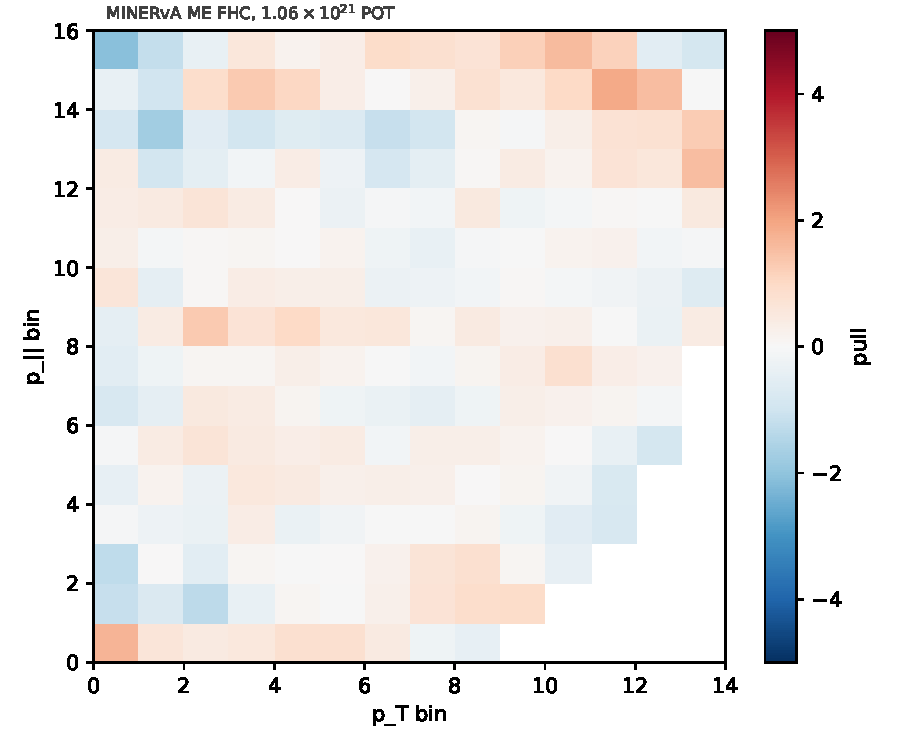
\includegraphics[width=\linewidth]{paper_validation_residual}
  \end{minipage}\hspace{1.2em}
  \begin{minipage}[c]{0.30\textwidth}
    \centering\footnotesize
    \textbf{Median relative uncertainty}\\[0.35em]
    \begin{tabular}{@{}lr@{}}
      This work & \SI{\uqMedian}{\percent} \\
      Published & \SI{\uqPaper}{\percent}
    \end{tabular}\\[0.8em]
    \textbf{Published-$\sigma$ standardized residuals}\\[0.35em]
    mean $=\pullMean$, RMS $=\pullRMS$
  \end{minipage}
  \caption{End-to-end validation against the published binned result
  \cite{MINERvA:2021owq}.  Top: $\pT$ and $\pPar$ projections of the published
  result, the five-iteration OmniFold result, and the MINERvA Tune~v1.  The two
  measurements use the same data, so their overlay validates the estimator
  rather than comparing independent results.
  Bottom left: $(\mathrm{OmniFold}-\mathrm{published})/\sigma_{\mathrm{published}}$
  on the reported two-dimensional grid; it is a descriptive shared-data
  residual, not an independent-result pull.  Bottom right: the independently
  reconstructed and published median relative uncertainties.}
  \label{fig:validation}
\end{figure*}

For the higher-dimensional results, every central-value construction is tested
against its lower-dimensional predecessor.  The three-, four-, and
five-observable marginal normalizations agree at the approximately
$1$--$2\%$ level, and injected distortions in each newly added variable are
recovered in closure tests.  These closure tests reweight the simulated signal
and do not exercise the background subtraction.  End-to-end pseudo-experiments
that include the purity-based background subtraction reproduce the input at
nominal truth except in the highest-$W$ cells, which are biased by up to
\SI{4}{\percent} in simulation, about one quoted standard deviation in one
$(\Eavail,W)$ cell; this bias is not included in the quoted uncertainties.
% Source: docs/orchestration/OUTCOME-20260925-s5c-purity-background-bias-at-high-W.md
% (D1: EW5-EW35 -3.5% to -4.1%, EW41 +1.66%); size vs adopted sigma:
% docs/orchestration/state/s5c/d1/bias_vs_adopted.json (max |bias|/sigma 1.07, EW35). KNOWN_ISSUES 75.

The $\Eavail$ dimension provides an independent view of the established
low-recoil discrepancy.  GENIE, the MINERvA Tune~v1, NuWro, and GiBUU all
underpredict the unfolded central value at low $\Eavail$.  Pion final-state
interaction variations change $d\sigma/d\Eavail$ by less than one percent,
whereas the empirical Valencia two-particle--two-hole contribution fills the
quasielastic--$\Delta$ dip. These tests constrain the chosen pion-FSI variations,
not all nuclear-transport models. Quasielastic-like measurements show sensitivity
to proton and pion FSI~\cite{MINERvA:2026qeleme}; their different signal definition
precludes identifying that effect with the inclusive discrepancy here.
Adding $q_{3}$ resolves the momentum-transfer
dependence of this feature.  On the maximal common $(\Eavail,q_{3})$ grid, the
central value agrees to within \SI{10}{\percent} with the dedicated published
low-recoil measurement~\cite{MINERvA:2022incl}.

The fifth observable, $W$, separates the remaining discrepancy from the
low-mass enhancement.  Figure~\ref{fig:joint} shows the joint
$(\Eavail,W)$ projection relative to the MINERvA Tune~v1, the tuned GENIE~2.12.6 simulation from which the unfolding starts.  The positive central-value
difference is concentrated where both $\Eavail$ and $W$ are large, rather than
being distributed uniformly across either one-dimensional projection.  Neither
one-dimensional projection resolves this structure.

\begin{figure}[t]
  \centering
  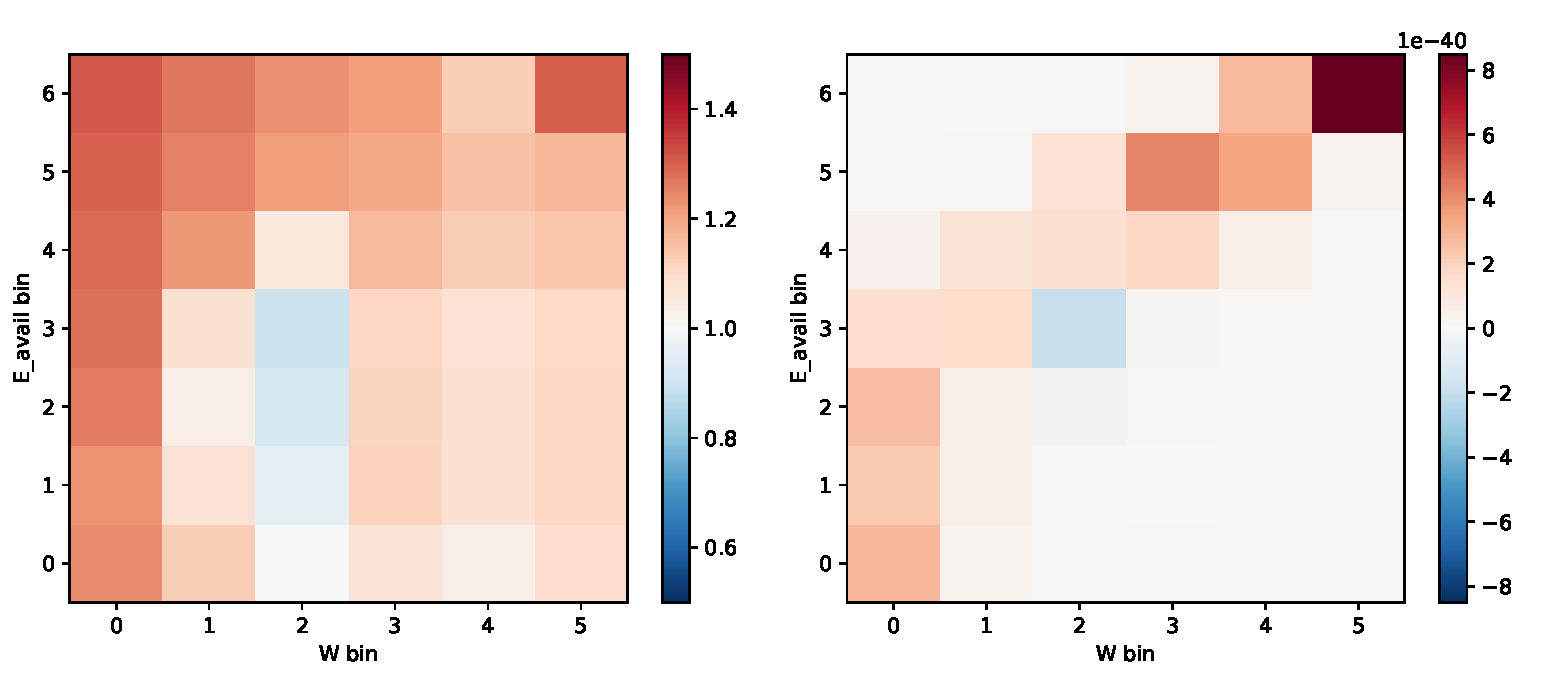
\includegraphics[width=\columnwidth]{paper_joint_localization}
  \caption{Localization in the joint $(\Eavail,W)$ central value, on the
  $7\times6$ reporting grid with $\Eavail$ edges
  $[0,0.1,0.2,0.4,0.8,1.5,3.0,100]\,\si{GeV}$ and $W$ edges
  $[0,1.1,1.4,1.8,2.2,3.0,100]\,\si{GeV}$; axes are cell indices counting from
  zero, so index~6 in $\Eavail$ and index~5 in $W$ are wide catch bins.  Left:
  the unfolded-to-Tune~v1 ratio per cell, dimensionless, on a $0.5$--$1.5$
  scale.  Right: the unfolded-minus-Tune~v1 difference as a
  \emph{cell-integrated} cross section in \si{cm^2/nucleon}, i.e.\ the
  density difference multiplied by that cell's
  $\Delta\Eavail\,\Delta W$; the catch-bin cells therefore carry their large
  widths and appear larger here than the ratio panel alone would suggest.  Read
  together, the panels put the remaining positive difference in the
  high-$\Eavail$, high-$W$ corner.  No significance is assigned.  The comparator is the MINERvA Tune~v1 (GENIE~2.12.6 with the analysis tune weights), not the untuned GENIE central value of Fig.~\ref{fig:generator-context}.}
  \label{fig:joint}
\end{figure}

The one-dimensional projections in Fig.~\ref{fig:generator-context} compare
the same central result with the four predictions that figure plots: GENIE's
own central value, the same GENIE with the Valencia two-particle--two-hole
component added, NuWro, and GiBUU.  All four underpredict the high-$W$ region.
Turning on the Valencia two-particle--two-hole component does not remove that
difference because it primarily populates lower $W$ --- visible here precisely
because the first two curves are two configurations of one generator rather
than independent predictions.  That several distinct generators agree on the
direction of the discrepancy is a useful model diagnostic.
Dedicated MINERvA shallow-inelastic measurements also report generator
disagreements~\cite{MINERvA:2025sis}, motivating differential tests across the
resonance--DIS transition. Their different selections preclude treating them as
independent confirmation of this localized difference.

\begin{figure*}[t]
  \centering
  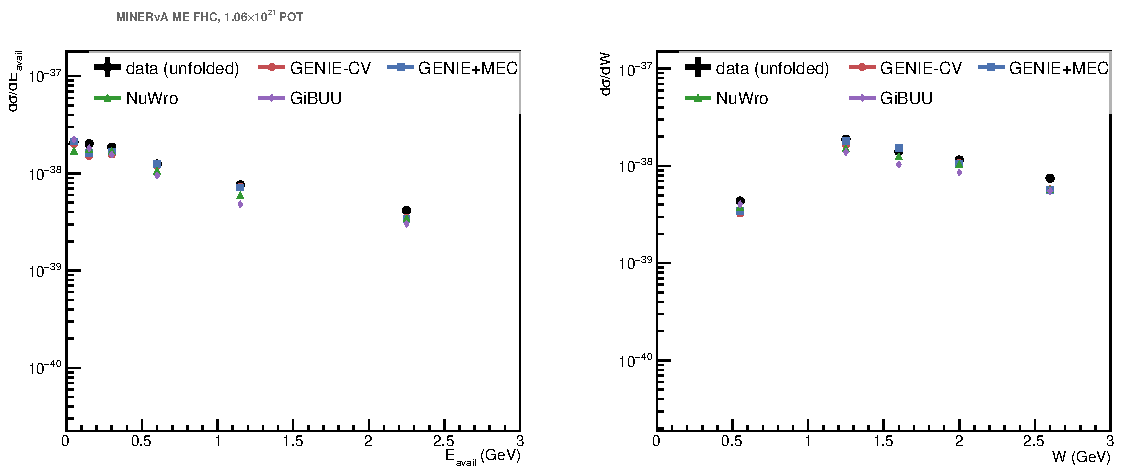
\includegraphics[width=0.84\textwidth]{paper_eavailW_generators}
  \caption{Generator context for the unfolded $\Eavail$ (left) and $W$ (right)
  central-value projections.  GENIE-CV (untuned GENIE~2.12.10 on CH, with no two-particle--two-hole events), the same GENIE with the Valencia two-particle--
  two-hole contribution, NuWro~21.09, and GiBUU~2019 (both on carbon) all remain below the unfolded result
  at high $W$.  No significance is assigned.}
  \label{fig:generator-context}
\end{figure*}

These results demonstrate that an unbinned event-weight construction can be
validated against an established two-dimensional measurement and extended to
five simultaneous observables.  The higher-dimensional central values recover
the known low-recoil behavior and expose a localized high-$\Eavail$, high-$W$
generator deficit.  Every non-two-dimensional result in this Letter is a
central value.  A scalar five-dimensional covariance is adopted under a
digest-bound exception, and its \zprojCells-cell $(\Eavail,W)$ projection is
built; no superseded or historical covariance is used here.  We nevertheless
quote no publication-level significance, and the reason is measured rather
than precautionary.  In a dedicated campaign of two companion covariances built at two estimator-seed settings for this test (products distinct from the adopted bytes), varying the seed moves the projected
uncertainty by \SI{\sprojMeasured}{\percent}, against a
\SI{\sprojBound}{\percent} movement limit fixed before production.  That
movement did not fall with ensemble size over the range tested:
\SI{\seedEffectNforty}{\percent} averaged over four disjoint 40-throw subsets,
\SI{\seedEffectNeighty}{\percent} over the two 80-throw halves, and
\SI{\sprojMeasured}{\percent} on the full 160-throw ensemble, fitted exponent
$\seedEffectExponent$.  A same-seed resampling floor, measured at $N=40$ and
$N=80$, falls steeply over that step --- \SI{\floorNforty}{\percent} to
\SI{\floorNeighty}{\percent}, two-point exponent $\floorExponent$.
Statistical noise must fall with $N$; this did not fall between $N=40$ and
$N=160$, so the failing leg is not reporting the statistic's own resampling
noise.  The comparison is a single seed pair and the 40- and 80-throw points
are nested subsets of the same 160 throws, so the width of the seed-pair
distribution and the behaviour at much larger $N$ are both unmeasured; the
statistic is a maximum over the declared offset set, so further pairs can only
raise it.  Five of the covariance's 45 bands are
built at a fixed seed the variation cannot reach, carrying
\SI{\pinnedBandsSqrtTr}{\percent} of $\sqrt{\mathrm{Tr}\,C}$ and contributing
none of the movement, so their seed sensitivity is unprobed and the effect on
the total were they also to vary is not measured in either direction.  The same variation
moves the projected central values by at most
\SI{\cvMoveOverSigmaMax}{\percent} of their own quoted uncertainty (median
\SI{\cvMoveOverSigmaMed}{\percent}).

The selection-complete replacement underlying that covariance covers the five
detector bands implemented through shifted reconstructed kinematics.  MINOS
efficiency and the three GEANT hadron-interaction bands retain their
weight-based treatment.  This classification establishes their exclusion from
the kinematic replacement; it does not independently validate the completeness
of the hadronic-response model for the $\Eavail$ and $W$ measurement.

Two extensions lie outside this result.  Removing the published truth-level
muon cuts gives a preliminary extended-fiducial cross section in which
detector-supported and prior-dominated regions are reported separately.  A
full-event point-cloud classifier could replace the scalar learner while
preserving the two-step pairing; it remains method development because the
nominal/statistical pairing was declined, coverage has not been demonstrated,
and no point-cloud uncertainty product is adopted.  Both extensions are
documented in the companion analysis note.


\begin{acknowledgments}
We thank the MINERvA Collaboration for making the data products used in this
study publicly available.
\end{acknowledgments}

\bibliographystyle{apsrev4-2}
\bibliography{technote}

\end{document}
